As the sun went down, the guests who were walking around the city started coming back to the hotel. The walrus was at the front desk, his long whiskers drooping. ``My pipe is gone!'' he bellowed. ``It was a gift when I became an honorary member of the Arctic Bocce Club.'' The owl hooted in dismay, clutching a photo of his grandfather. ``My monocle is gone! It's the only item I have to remember him by!'' The giraffe cried that her red scarf had vanished. ``It's the only souvenir from my first time skiing in the Himalayas!'' The rabbit bounced up and down, looking for his wristwatch. ``I desperately need my wristwatch! How can I tell when it's time for my medicine?!'' The pig was sweating in anxiety. ``My football match is about to start!'' And right behind him stood a bear, who clutched his pants with his paws. ``My suspenders are gone!'' he growled. ``How will my pants stay up without them?''

The giraffe, visibly upset, added, ``We need to find the thief! They can't steal our valuables and get away with it!'' Her frustration was echoed by the others, all eager to solve the crime.

The rabbit, taking advantage of everyone's resolve, pointed out, ``When I went down to the pharmacy, I saw the wolf wandering the stairs and hallways.'' Just then, the wolf appeared, and with a choking cough, he loudly said, ``Cough! Hey! I'm a victim here too! I was wandering around looking for my spa voucher, which I won at the reception!''

Henrietta quickly intervened, asking everyone to calm down. ``Mr. Wolf was indeed awarded a spa voucher upon arrival.''

Then the ostrich appeared, holding a ticket in its beak. ``I think I found your voucher, Mr. Wolf.''

\begin{center}
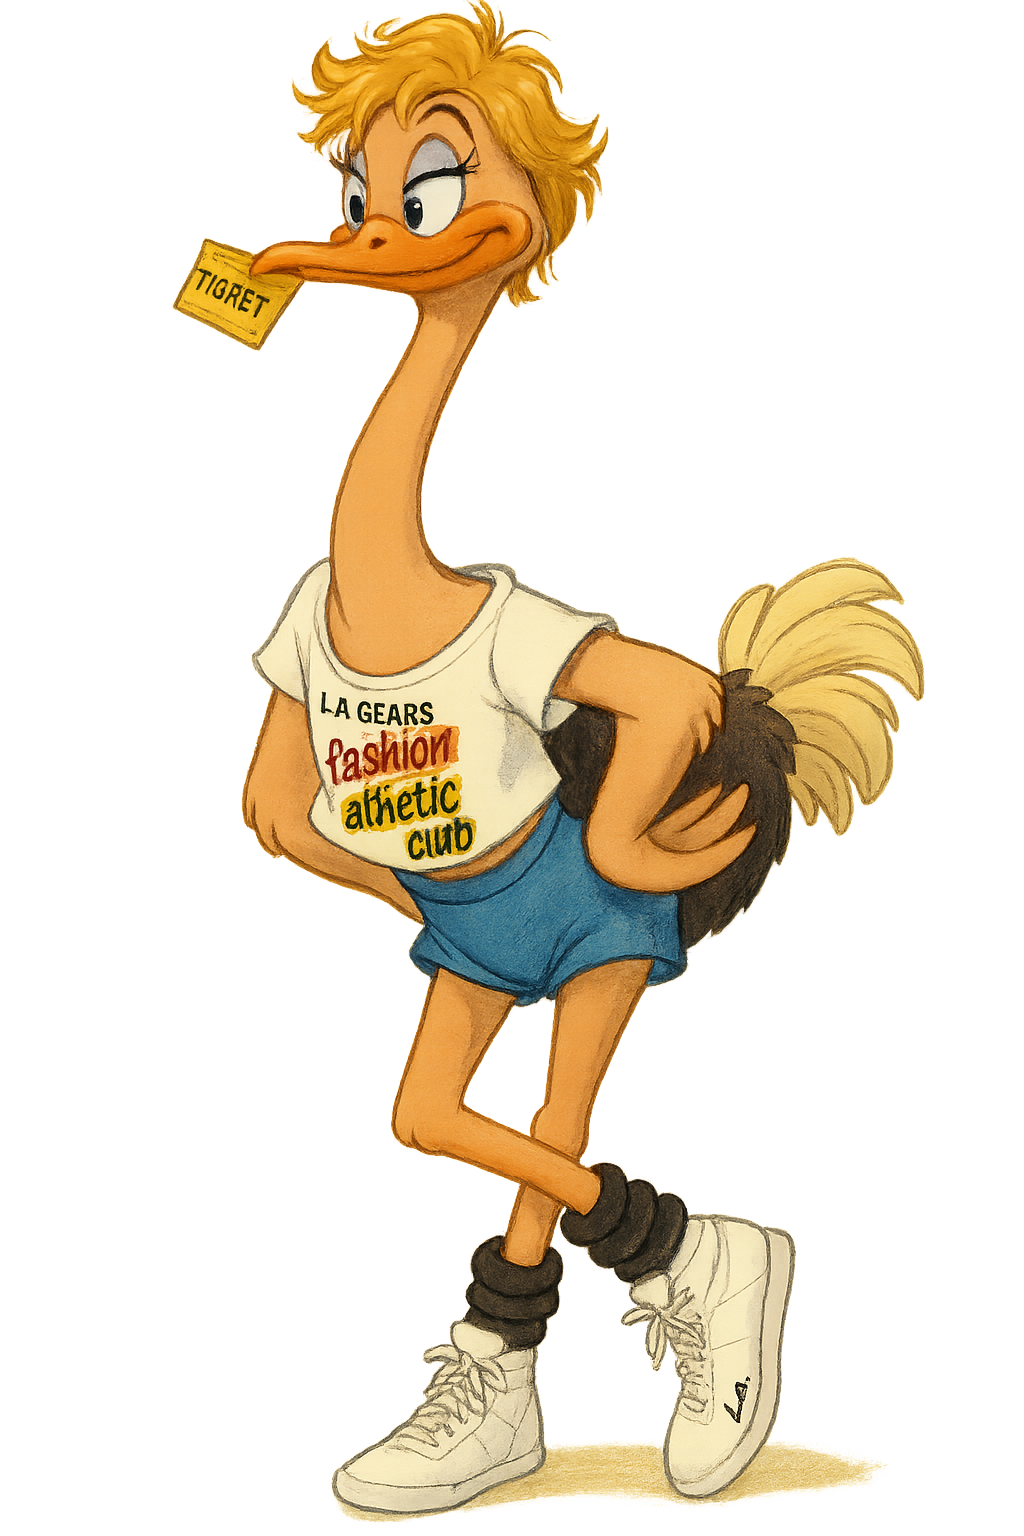
\includegraphics[width=0.4\textwidth]{images/ostrich.png}
\end{center}

The rabbit, with a sly look, pointed out, ``We can then conclude that the wolf was not a victim of the disappearances...''

The animals began to turn on each other. The owl accused the rabbit of being too shifty and quick-witted. She added, ``He's pointing the finger at the wolf to take the focus off himself.'' The rabbit retorted, ``That's a frivolous accusation!'' Just then, a rooster with a red comb took advantage of the confusion and crowed loudly: ``Don't trust her!'' He pointed his wing at the fox, accusing her of being very cunning and sneaky. The fox, in turn, pointed her paw at the pig, claiming he was clumsy and messy. The pig, frustrated, simply snorted in disbelief.

When the commotion reached a fever pitch, a girl named Anne arrived with her fluffy Border collie, Scotch. She listened carefully to the animals' stories while Scotch, on the other hand, was sniffing everything.

``We can help,'' Anne said confidently. ``Scotch can follow the trail of your missing items.''

The fox and the wolf exchanged a sly look. ``Why don't you start with the rabbit's room?'' the fox suggested. ``He seems awfully nervous.''

``Go ahead!'' the rabbit exclaimed, puffing out his chest. ``You can see my room. I have nothing to hide, and you'll be disappointed!''

\clearpage
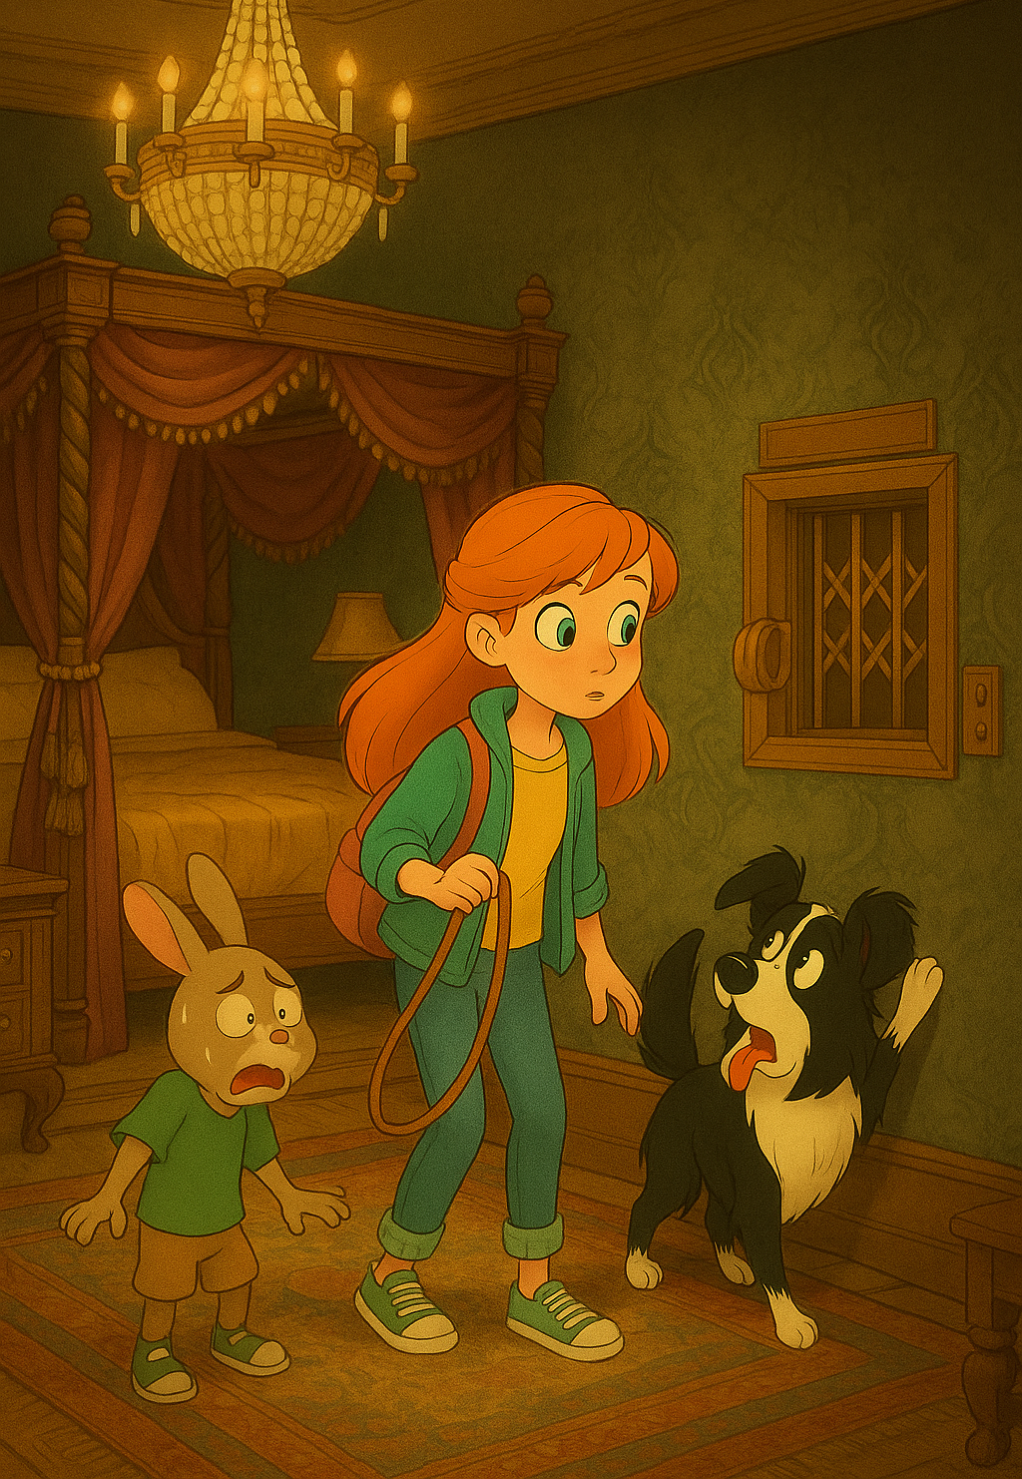
\includepdf[pages={1},
            pagecommand={\thispagestyle{fancy}}, % Apply your custom 'fancy' style
            fitpaper=true,
            noautoscale
           ]{rabbitpanic.pdf}

They all went to the rabbit's room. Scotch began smelling everything: the door, the floor, the wardrobe... and suddenly they saw a shiny monocle lying on the floor, next to the freight elevator. The wolf let out a satisfied snort. ``Well, it looks like we found what we were looking for.''

The rabbit stammered, ``I don't know how this got here!'' He broke out in a cold sweat, turned pale, and looked as if he was about to faint.

But Scotch barked once again. He stood on his hind legs, his front claws gripping the wall for support. With his nose raised high, he eagerly sniffed the elevator, his body tense with curiosity and excitement.

``It seems the trail leads to this small elevator,'' Anne added. ``Where does it go?''

Bernard responded promptly, ``It goes to every room in the hotel.''

Henrietta added, ``But there are an infinite number of rooms... it will take forever to find the lost items!''

Scotch barked again and started pulling Anne out of the room. He led her down the hallway to a room service cart that was parked in the middle of the corridor. A white cloth covered the items on the lower shelf, but Scotch's nose was working overtime. With the curious dog sniffing intently, Anne gently lifted the cloth to see what lay underneath.

\newpage
She was surprised to find a jar full of dog biscuits. She laughed, ``Haha! Scotch, you have a sweet tooth!''

Just then, Bernard approached, opened the jar, and gave him three biscuits. Scotch barked, as if to thank him for the treat.

%\begin{center}
%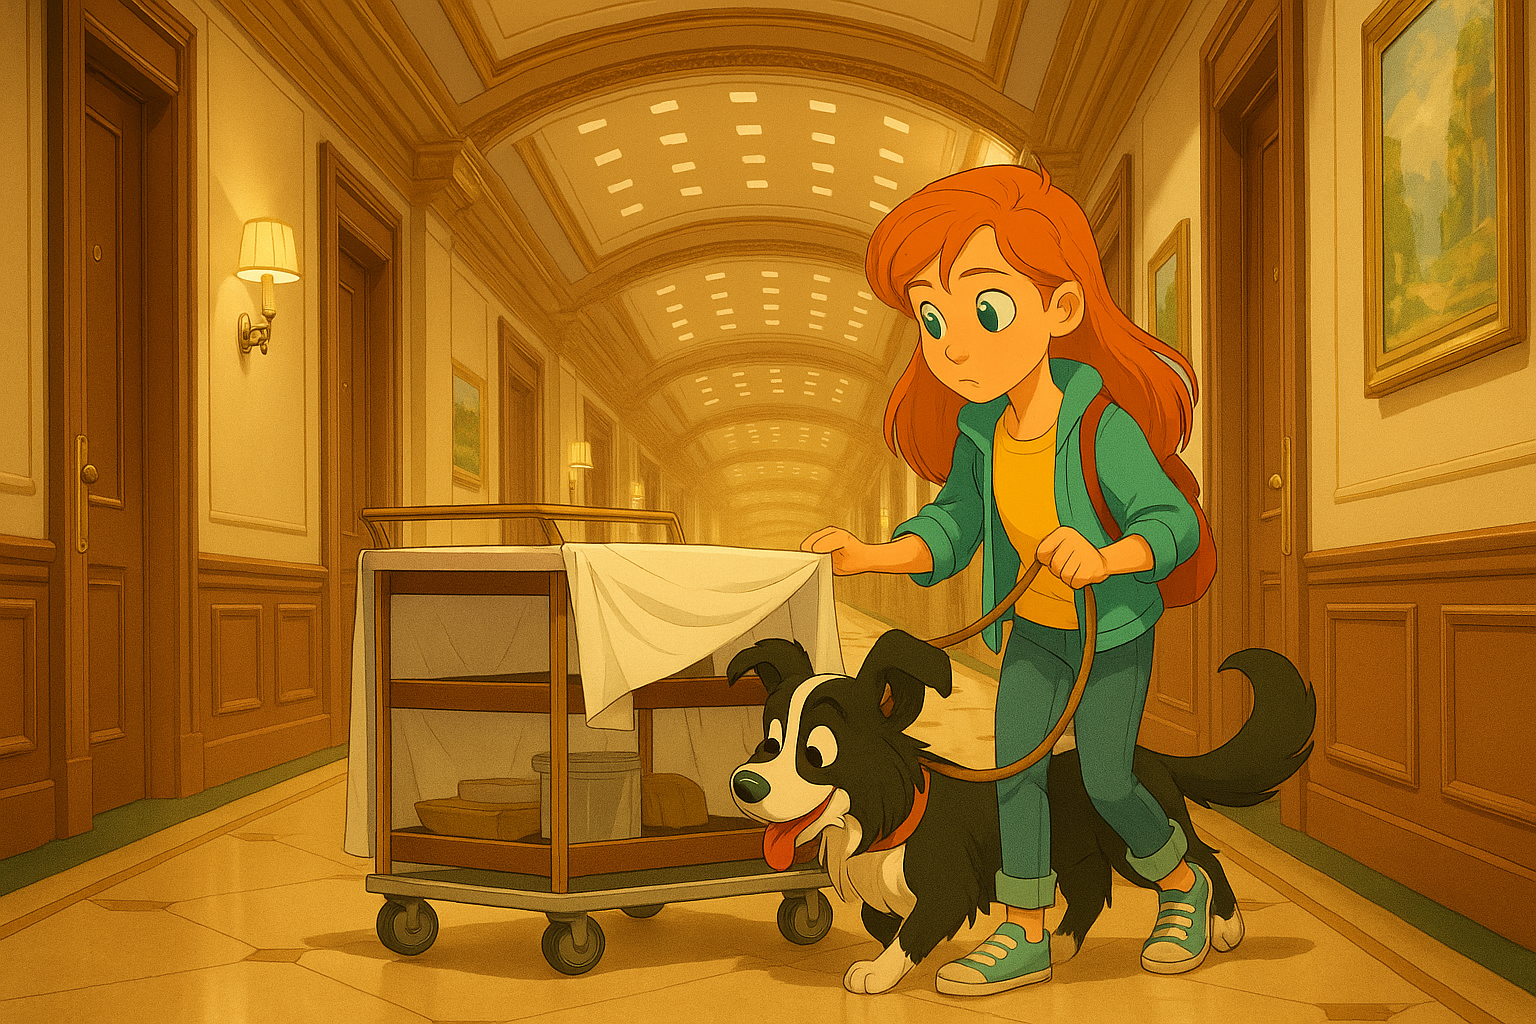
\includegraphics[width=0.65\textwidth]{images/biscuits.png}
%\end{center}

%After his well-earned snack, Scotch then bolted back toward the lobby, with the whole group following close behind him. He found another door for the freight elevator, sat down, and barked.
After his well-earned snack, Scotch led the group as they searched room after room, but they couldn't find a single clue. As the animals' hope began to fade, the sheer impossibility of the task -- to find the missing items in a myriad of rooms -- set in. Just as they were turning back toward the lobby, Scotch found another door for the freight elevator, sat down, and barked.
Anne looked from the door to the group of animals, a spark of understanding in her eyes. ``I think I see now,'' she said. ``This door leads to the same elevator, doesn't it?''

Bernard immediately added, ``Indeed! To move the guests' belongings, we needed to use this entrance for the elevator so that we may choose to which room to send them.''
\clearpage
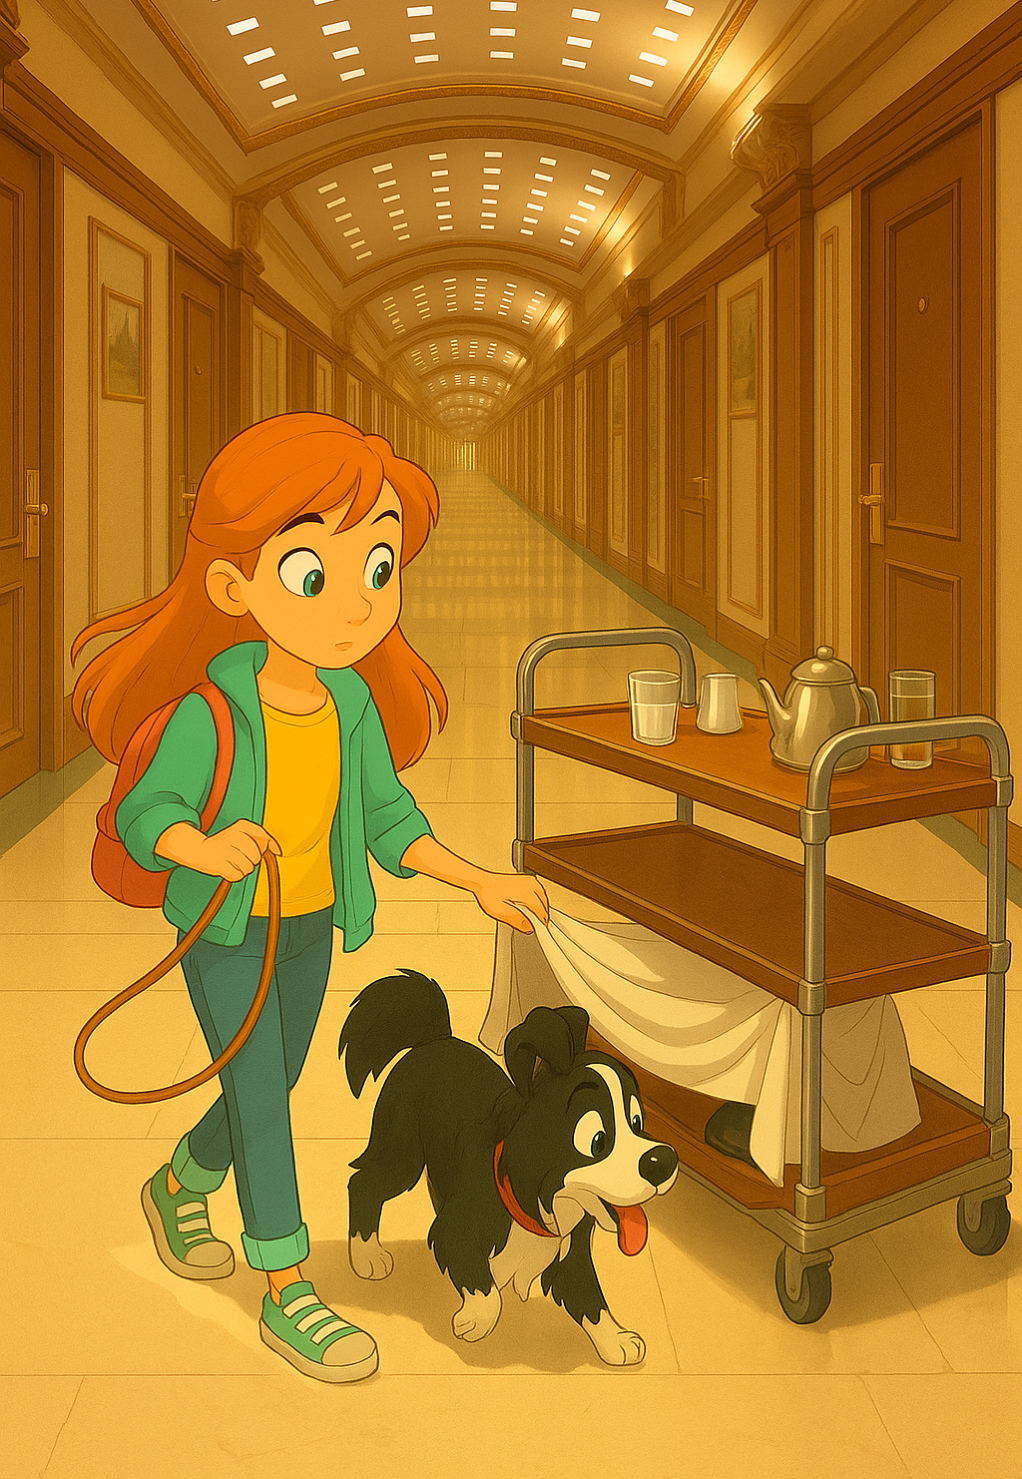
\includepdf[pages={1},
            pagecommand={\thispagestyle{fancy}}, % Apply your custom 'fancy' style
            fitpaper=true,
            noautoscale
           ]{biscuit.pdf}


\clearpage

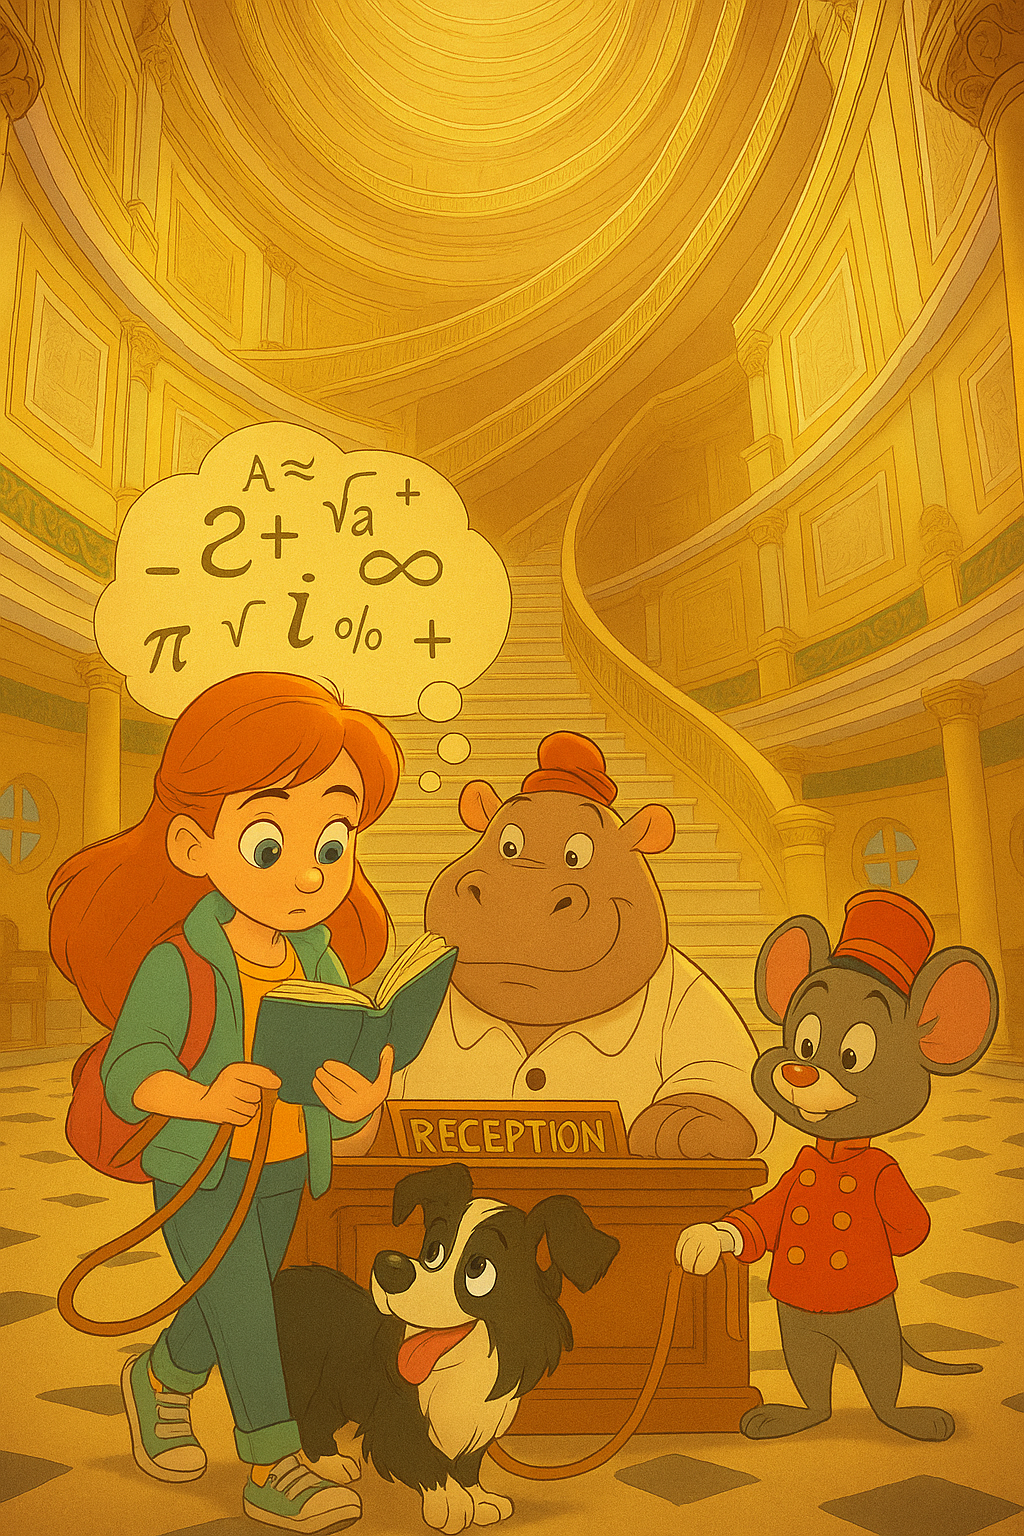
\includepdf[pages={1},
            pagecommand={\thispagestyle{fancy}}, % Apply your custom 'fancy' style
            fitpaper=true,
            noautoscale
           ]{manual.pdf}

Anne thoughtfully pointed out, ``It's starting to become clear. We just need to find the intricate workings of the elevator system.''

Bernard asked, ``Do we have a map for the elevator system?''

Henrietta explained they only had a manual, and Anne remarked, ``There might not be such a map, or it would be infinitely large!'' Bernard almost laughed and said, ``I will go look for the manual. I will be right back!''

Bernard quickly came back with the manual in his hands. He delivered it to Anne, who immediately started flipping through its pages. ``Ah! I found it!'' she exclaimed with excitement. ``The engineers used a Cantor's Pairing Function to map the room number and floor with the position of the elevator on its infinite track.'' 
She showed Henrietta a formula in the book, explaining how it performed the mapping. % mapped the room number and floor to a single number that told the elevator where to go. 
She also warned, ``We need to remember the index here starts with zero!''
%She showed Henrietta a formula in the book: $n=(i+j)(i+j+1)/2+j$. Anne explained, ``$n$ is the elevator position, $i$ is the room number, and $j$ is the floor.'' She also warned, ``We need to remember the index here starts with zero!''

Everybody looked at Anne with relief, despite not being able to understand any of the math. She opened her bag and took out a scientific calculator. After a few keystrokes, she exclaimed: ``I got it! Let's go, Scotch! Let's find the missing heirlooms!''
